\section{Conception — PSM}

\subsection{Choix technologiques}

L'expérience croisée des \emph{BackSynth Boys} nous a conduit à
nous tourner vers le \emph{framework} Qt, dont chacun apprécie
l'API élégante et performante. Ce framework fournit surtout des
outils pour la construction d'interfaces homme-machine, mais il est
très riche et possède également des APIs pour la manipulation de
collections, ou le traitement de documents XML.

La meilleure façon de tirer parti de Qt est de programmer en C++,
c'est donc le langage qui a été choisi pour le développement de
SynthPro.

\subsection{Conséquences sur l'architecture}

\subsubsection{Diagramme de classes de niveau PSM}

\begin{figure}[htb]
\centering
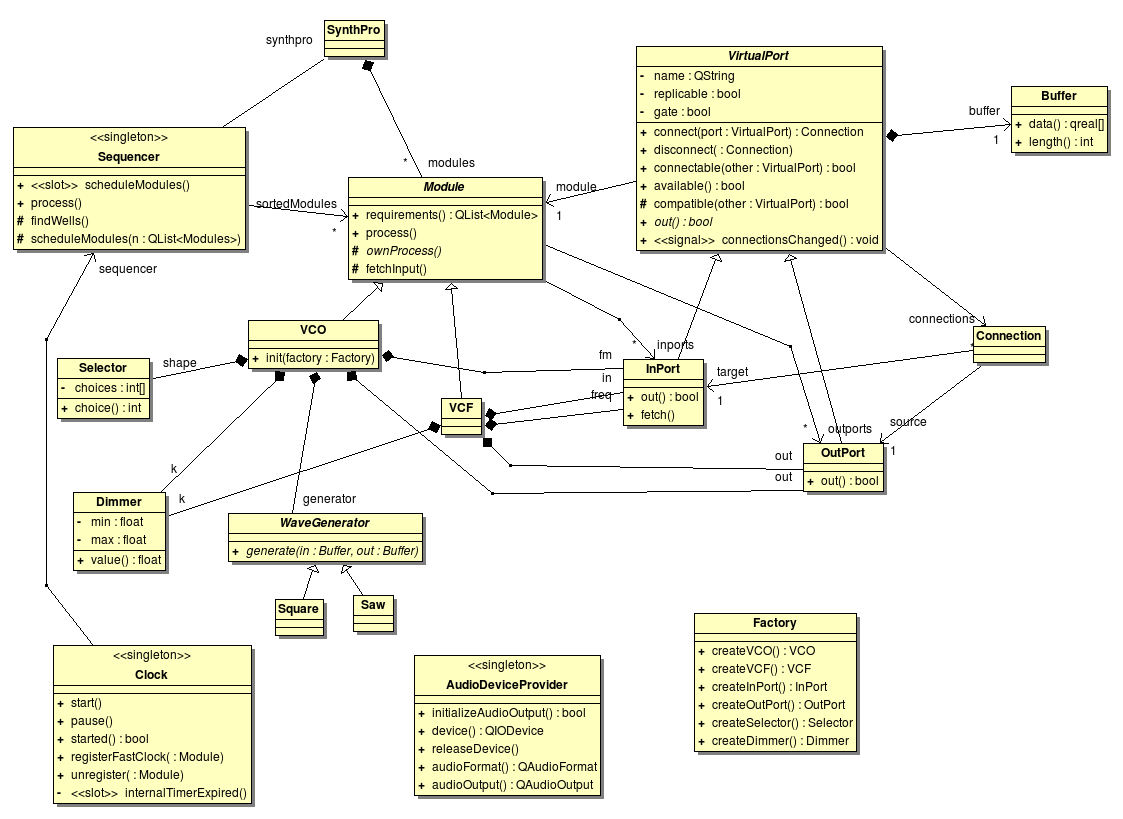
\includegraphics{https://github.com/iMax-pp/SynthPro/raw/master/doc/img/png/business-psm.png}
\caption{Figure n — Classes métier au niveau PSM}
\end{figure}

La figure n représente les classes métier au niveau PSM. Il n'y a
pas vraiment de changement profond par rapport au niveau PIM, les
types de données de Qt sont utilisés (\verb!QList!, \verb!QString!,
etc.), et des \emph{signals} et \emph{slots} apparaissent. Un
\emph{signal} est une notification qu'un composant émet pour
informer d'un événement, un \emph{slot} est une opération
(\emph{handler}) qui peut être appelée pour gérer cette
notification. Le système de \emph{signals} et \emph{slots} est une
implémentation proposée par Qt du patron de conception
\emph{Observer}.

Par exemple, la classe \verb!VirtualPort! émet le signal
\verb!connectionsChanged! à chaque fois qu'une connexion ou une
déconnexion a lieu. Ce signal est intercepté par le \verb!SynthPro!
qui demande au \verb!Sequencer! de recalculer l'ordonnancement de
ses modules.

Enfin, la classe \verb!AudioDeviceProvider! fait son apparition,
elle gère l'accès à la carte son en utilisant l'API QtMultimedia.

\subsubsection{Héritage en diamant}

\begin{figure}[htb]
\centering
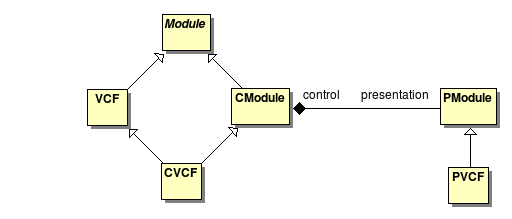
\includegraphics{https://github.com/iMax-pp/SynthPro/raw/master/doc/img/png/pacmodule-psm.png}
\caption{Figure n — Losange}
\end{figure}

Notre choix de faire hériter les contrôles des composants de leur
abstraction a conduit à un problème d'héritage en diamant. Nous
avons donc pu goûter aux joies de l'héritage virtuel en C++ et de
ses effets pervers.

\subsection{Conséquences sur la gestion du son}

[[PSM - Le moteur audio]]

\subsection{Conséquences sur l'interface utilisateur}

Nous avons utilisé le \emph{framework} GraphicsView de Qt pour
gérer l'affichage des modules. Ce \emph{framework} est conçu pour
afficher des objets 2D dans une scène très efficacement.

